\documentclass[12pt,a4paper]{article}
\usepackage[T1,T2A]{fontenc}
\usepackage[utf8]{inputenc}
\usepackage[english,russian]{babel}
\usepackage{microtype}
\usepackage{csquotes}
\usepackage{amsmath}
\usepackage{amsthm}
\usepackage{amssymb}
\usepackage{mathtext}
\usepackage[notrig,italicdiff]{physics}
\usepackage{newfloat}
\usepackage{caption}
\usepackage{indentfirst}
\usepackage{geometry}
\usepackage{hyperref}
\usepackage{mdframed}
\usepackage[inline]{enumitem}
\usepackage{graphicx}
\usepackage{subfig}
\usepackage{titlesec,titletoc}
\usepackage[titletoc,title]{appendix}
\geometry{left=3cm,right=2cm,top=2cm,bottom=2cm}
\DeclareGraphicsExtensions{.pdf,.png,.jpg,.PNG}
\graphicspath{{./img/}}
\captionsetup[figure]{justification=centering}
\renewcommand{\thesubfigure}{\asbuk{subfigure}}
\DeclareCaptionLabelSeparator{dotseparator}{. }
\titlelabel{\thetitle. }
\patchcmd{\appendices}{\quad}{. }{}{}
\captionsetup{labelsep=dotseparator}
\hypersetup{
	colorlinks,
	citecolor=black,
	filecolor=black,
	linkcolor=black,
	urlcolor=black
}

\begin{document}

    \newcommand\blanktextfield[2]{$\underset{\text{#1}}{\text{\underline{\hspace{#2}}}}$}

\makeatletter
\begin{titlepage}

	\large\newpage

    \noindent\centering{
    	МИНИСТЕРСТВО ОБРАЗОВАНИЯ И НАУКИ РОССИЙСКОЙ ФЕДЕРАЦИИ

    	Федеральное государственное автономное образовательное учреждение высшего образования \enquote{Национальный исследовательский Нижегородский государственный университет им. Н.И. Лобачевского}
    }

	\vspace*{50pt}

	Физический факультет \\[\baselineskip]

	Кафедра информационных технологий\\
	в физических исследованиях

	\vspace*{\fill}

	{\Large\textbf{Определение энергии образования вакансии в кремниевом кристалле при межатомном потенциале взаимодействия Стиллинджера-Вебера}}

	\vspace*{\fill}

	\hfill\begin{minipage}{22em}
    	Отчет по лабораторной работе\\
		студента 1 курса магистратуры 05182 группы\\
		\textbf{Василевского А.В.}
    \end{minipage} \\[\baselineskip]

	\hfill\begin{minipage}{22em}
		Основная профессиональная образовательная
		программа подготовки магистров по
		направлению 09.04.02~--- \enquote{Информационные системы и технологии}
		(профиль программы: \enquote{Информационные системы и технологии в физических исследованиях})
    \end{minipage}

	\vspace*{\fill}

	\hfill\begin{minipage}{15em}
		\blanktextfield{(подпись)}{1in} Василевский А.В.\\[\baselineskip]
		Руководитель учебной практики:\\
		доцент кафедры ИТФИ\\
		к. ф.-м. н.\\[\baselineskip]
		\blanktextfield{(подпись)}{1in} Васин А.С.
    \end{minipage}

	\vspace*{\fill}

	Нижний Новгород\\
	2018

\end{titlepage}
\makeatother


    \tableofcontents

    \clearpage

    %
    %
    %
    %%%%%%%%%%%%%%%%%%%%%%%%%%%%%%%%%%%%%%%%%%%%%%%%%%%%%%%%%%%%%%%%%%%%%%%
    %                           SECTION                                   %
    %%%%%%%%%%%%%%%%%%%%%%%%%%%%%%%%%%%%%%%%%%%%%%%%%%%%%%%%%%%%%%%%%%%%%%%
    %
    %
    %

    \section{Постановка задачи}

        Применить метод молекулярной динамики с потенциалом Стиллинджера-Вебера к задаче нахождения энергии образования вакансии в кристалле кремния.

    %
    %
    %
    %%%%%%%%%%%%%%%%%%%%%%%%%%%%%%%%%%%%%%%%%%%%%%%%%%%%%%%%%%%%%%%%%%%%%%%
    %                           SECTION                                   %
    %%%%%%%%%%%%%%%%%%%%%%%%%%%%%%%%%%%%%%%%%%%%%%%%%%%%%%%%%%%%%%%%%%%%%%%
    %
    %
    %

    \section{Физическая модель}

        Рассматривается некоторая конечная область кристалла кремния. При этом считается, что вакансия образуется на месте центрального атома. Энергия образования вакансии~--- разность между начальной (без вакансии) и конечной (с вакансией) энергией системы (с поправкой на энергию \enquote{лишнего} атома).

        Переход из начального состояния в конечное осуществляется при помощи метода молекулярной динамики с определенным потенциалом, параметры которого берутся из специальных таблиц.

    %
    %
    %
    %%%%%%%%%%%%%%%%%%%%%%%%%%%%%%%%%%%%%%%%%%%%%%%%%%%%%%%%%%%%%%%%%%%%%%%
    %                           SECTION                                   %
    %%%%%%%%%%%%%%%%%%%%%%%%%%%%%%%%%%%%%%%%%%%%%%%%%%%%%%%%%%%%%%%%%%%%%%%
    %
    %
    %

    \section{Математическая модель}

        %
        %
        %
        %%%%%%%%%%%%%%%%%%%%%%%%%%%%%%%%%%%%%%%%%%%%%%%%%%%%%%%%%%%%%%%%%%%
        %                        SUBSECTION                               %
        %%%%%%%%%%%%%%%%%%%%%%%%%%%%%%%%%%%%%%%%%%%%%%%%%%%%%%%%%%%%%%%%%%%
        %
        %
        %

        \subsection{Метод молекулярной динамики}

            Метод молекулярной динамики относится к классу методов многочастичного моделирования. Динамика системы частиц описывается при помощи системы дифференциальных уравнений Ньютона, при этом потенциал взаимодействия частиц заранее выбирается из каких-либо соображений и постулируется.

            В декартовой системе координат $6N$ уравнений, описывающих динамику $N$ частиц, могут быть записаны в следующей однородной форме:
            %
            \begin{equation*}
                \dot{\vb{x}}_i = \vb{v}_i, \quad
                \dot{\vb{v}}_i = \frac{\vb{F}_i}{m_i} , \quad
                i \in [1,N]
            \end{equation*}
            %
            При этом сила $\vb{F}_i$ вычисляется как
            %
            \begin{equation*}
                \vb{F}_i = - \nabla U(\vb{x}_i;\vb{x}_1,\dots,\vb{x}_N)
            \end{equation*}
            %
            Обычно рассматриваются двухчастичные и трехчастичные потенциалы: $U=U(\vb{x}_i;\vb{x}_j)$ и $U=U(\vb{x}_i;\vb{x}_j,\vb{x}_k)$. Для сложных потенциалов чаще бывает проще вычислять градиент численно (например, по формулам трехточечного дифференцирования).

            Метод молекулярной динамики не преследует цель максимально точно воспроизвести движение отдельных частиц. Главная задача метода~--- позволить по микроскопическим характеристикам отдельных частиц (координаты, скорости) судить о макроскопических характеристиках всей системы: энергии, плотности, давлении и т.д.

            При моделировании на компьютере для решения уравнений динамики чаще всего использую скоростную форму алгоритма Верле:
            %
            \begin{equation*}
                \vb{x}_i^{k+1} = \vb{x}_i^k + \vb{v}_i^k \Delta t + \frac{\vb{F}_i^k}{2m} \Delta t^2, \quad
                \vb{v}_i^{k+1} = \vb{v}_i^k + \frac{\vb{F}_i^k + \vb{F}_i^{k+1}}{2m} \Delta t,
            \end{equation*}
            %
            Начальные и граничные условия выбираются исходя из особенностей задачи. Так, в кристаллах начальные скорости частиц обычно полагают равными нулю: $\vb{v}_i^0 = 0$. Начальные координаты же определяются структурой решетки. Граничные условия в кристаллах могут быть двух видов: свободные и жесткие. В отличие от первого, в последнем случае положение граничных атомов жестко фиксируется.

            В целях уменьшения погрешностей компьютерных вычислений следует все уравнения привести к безразмерному виду.

            Шаг по времени следует выбирать из тех соображений, чтобы суммарная энергия системы со временем менялась не более чем на $\sim 1-2\%$.

        %
        %
        %
        %%%%%%%%%%%%%%%%%%%%%%%%%%%%%%%%%%%%%%%%%%%%%%%%%%%%%%%%%%%%%%%%%%%
        %                        SUBSECTION                               %
        %%%%%%%%%%%%%%%%%%%%%%%%%%%%%%%%%%%%%%%%%%%%%%%%%%%%%%%%%%%%%%%%%%%
        %
        %
        %

        \subsection{Потенциал Стиллинджера-Вебера}

            В ковалентных кристаллах потенциал взаимодействия атомов в решетке зависит не только от расстояния между частицами, но и от углов связей. Потому центральные двухчастичные потенциалы, как то потенциал Леннарда-Джонса, для них не годятся. Поэтому в таких кристаллах, как кремний, следует использовать трехчастичные потенциалы. Одним из таких потенциалов является потенциал Стиллинджера-Вебера.

            Потенциальная энергия взаимодействия $N$ атомов имеет вид:
            %
            \begin{equation*}
                U=\sum\limits_{i<j}^N U_2(\vb{r}_i,\vb{r}_j) + \sum\limits_{i<j<k}^N U_3(\vb{r}_i,\vb{r}_j,\vb{r}_k),
            \end{equation*}
            %
            где $\vb{r}_i$~--- радиус-вектор $i$-го атома. Первое слагаемое описывает двухчастичное взаимодействие, второе~--- трехчастичное взаимодействие.
            %
            \begin{equation*}
                U_2(\vb{r}_i,\vb{r}_j) = \varepsilon f_2(\rho_{ij}), \quad
                f_2(\rho_{ij}) = \Omega(\rho_{ij}) A \qty[
                    B \rho_{ij}^{-p} - \rho_{ij}^{-q}
                ] \exp\qty[(\rho_{ij}-\rho_1)^{-1}],
            \end{equation*}
            %
            \begin{equation*}
                U_3(\vb{r}_i,\vb{r}_j,\vb{r}_k) = \varepsilon f_3(\rho_{i},\rho_{j},\rho_{k}),
            \end{equation*}
            %
            \begin{equation*}
                f_3(\rho_{i},\rho_{j},\rho_{k}) = h(\rho_{ij},\rho_{ik},\theta_{jik}) + h(\rho_{ji},\rho_{jk},\theta_{ijk}) + h(\rho_{ki},\rho_{kj},\theta_{ikj}),
            \end{equation*}
            %
            \begin{equation*}
                h(\rho_{ij},\rho_{ik},\theta_{jik}) = \Omega(\rho_{ij}) \Omega(\rho_{ik}) \lambda \exp\qty[\gamma (\rho_{ij}-\rho_1)^{-1} + \gamma (\rho_{ik}-\rho_1)^{-1}] \qty(\cos\theta_{jik} + \frac{1}{3})^2 .
            \end{equation*}
            %
            Здесь $\rho=\flatfrac{r}{\sigma}$, $\sigma$, $\lambda$, $\varepsilon$, $\gamma$, $A$, $B$, $p$, $q$, $r_1$~--- параметры потенциала ($r_1$~--- радиус обрезания потенциала). $\Omega(\rho < \rho_1) = 1$, $\Omega(\rho) = 0$~--- индикаторная функция интервала $\rho \in (0,\rho_1)$. $r_{ij}$~--- расстояние между центрами $i$ и $j$ атома, $\theta_{ijk}$~--- угол между векторами $\vb{r}_{ij}$ и $\vb{r}_{ik}$. Параметр $\sigma$ выражается через параметр решетки $a$ следующим образом:
            %
            \begin{equation*}
                \sigma = \flatfrac{r_0}{\sqrt[6]{2}}, \quad r_0 = a \flatfrac{\sqrt{3}}{4} .
            \end{equation*}

    %
    %
    %
    %%%%%%%%%%%%%%%%%%%%%%%%%%%%%%%%%%%%%%%%%%%%%%%%%%%%%%%%%%%%%%%%%%%%%%%
    %                           SECTION                                   %
    %%%%%%%%%%%%%%%%%%%%%%%%%%%%%%%%%%%%%%%%%%%%%%%%%%%%%%%%%%%%%%%%%%%%%%%
    %
    %
    %

    \section{Численная модель}

        %
        %
        %
        %%%%%%%%%%%%%%%%%%%%%%%%%%%%%%%%%%%%%%%%%%%%%%%%%%%%%%%%%%%%%%%%%%%
        %                        SUBSECTION                               %
        %%%%%%%%%%%%%%%%%%%%%%%%%%%%%%%%%%%%%%%%%%%%%%%%%%%%%%%%%%%%%%%%%%%
        %
        %
        %

        \subsection{Начальное размещение частиц}

            В начальный момент времени частицы должны находиться в узлах кристаллической решетки. Наиболее простой способ добиться этого~--- генерировать решетку слоями, начиная от центрального атома.

            В кристалле кремния можно выделить простую элементарную кубическую ячейку из пяти атомов, четыре из которых расположены в вершинах куба, один~--- в его центре. Определив радиус-векторы атомов в вершинах куба относительно центрального атома, можно последовательно генерировать слои решетки методом откладывания векторов от данного атома, пока не будет достигнут необходимый объем расчетной ячейки.

        %
        %
        %
        %%%%%%%%%%%%%%%%%%%%%%%%%%%%%%%%%%%%%%%%%%%%%%%%%%%%%%%%%%%%%%%%%%%
        %                        SUBSECTION                               %
        %%%%%%%%%%%%%%%%%%%%%%%%%%%%%%%%%%%%%%%%%%%%%%%%%%%%%%%%%%%%%%%%%%%
        %
        %
        %

        \subsection{Вычисление энергии образования вакансии}

            Образование вакансии можно смоделировать удалением центрального атома из кристаллической решетки и последующей релаксацией образовавшейся неравновесной структуры методом молекулярной динамики.

            При этом для обеспечения схождения системы к стационарному состоянию следует отнимать избыточную кинетическую энергию. Сделать это можно, например, таким способом. Когда кинетическая энергия некоторого атома достигнет своего максимума, скорости всех частиц обнуляются.

            Энергию образования вакансии можно вычислить по следующей формуле:
            %
            \begin{equation*}
                E_V = E_\text{пот}^0 \frac{N-1}{N} - E_\text{пот} .
            \end{equation*}
            %
            Здесь $E_\text{пот}^0$ и $E_\text{пот}$~--- энергия системы до и после образования вакансии. Поправочный множитель $\flatfrac{N-1}{N}$ учитывает факт удаления атома.

    %
    %
    %
    %%%%%%%%%%%%%%%%%%%%%%%%%%%%%%%%%%%%%%%%%%%%%%%%%%%%%%%%%%%%%%%%%%%%%%%
    %                           SECTION                                   %
    %%%%%%%%%%%%%%%%%%%%%%%%%%%%%%%%%%%%%%%%%%%%%%%%%%%%%%%%%%%%%%%%%%%%%%%
    %
    %
    %

    \section{Анализ результатов}

        В ходе работы была написана демонстрационная программа (\autoref{fig:mainwindow}) на языке  \enquote{C++}, позволяющая рассчитать энергию образования вакансии в кристалле кремния.
        %
        \begin{figure}[h]
            \centering
            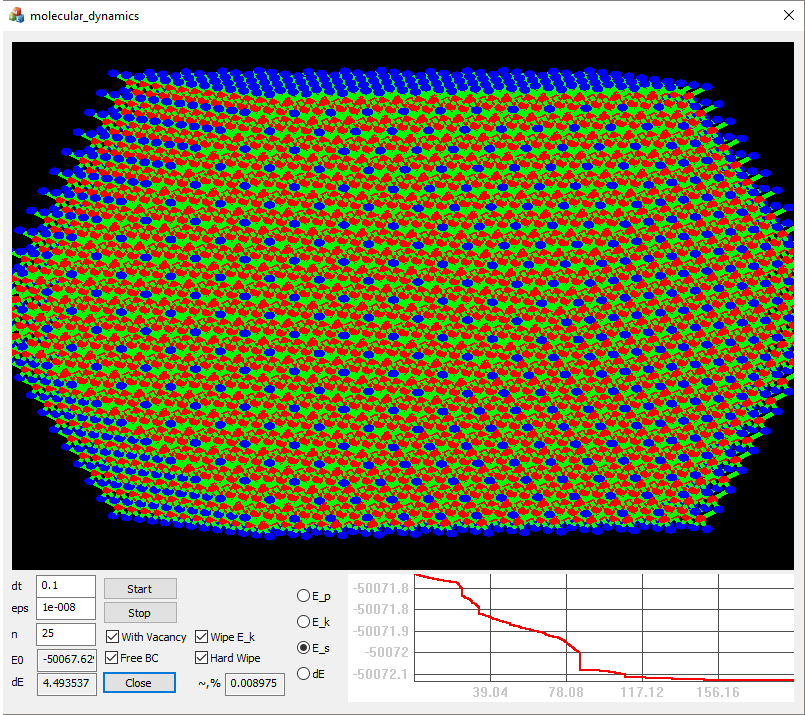
\includegraphics[width=0.8\textwidth]{mainwindow}
            \caption[]{Главное окно программы}
            \label{fig:mainwindow}
        \end{figure}
        %
        Программа отображает вид кристаллической решетки при заданном количестве слоев решетки. Динамику процесса релаксации системы можно отследить по графикам суммарных кинетической, потенциальной, полной энергии системы, а также вычисленной на текущем шаге по времени энергии образования вакансии. Отклонение полной энергии от ее первоначального значения можно проследить по числовому значению, отображаемому на главном окне. Программа также позволяет задать тип граничных условий (жесткие или свободные).

        На \autoref{fig:1}-\autoref{fig:2} показаны варианты кристаллической решетки кремния при разном количестве слоев.

        На \autoref{fig:2} приведены результаты моделирования для различных конфигураций системы.
        %
        \begin{figure}[!htb]%
            \centering
            %
            \subfloat[][]{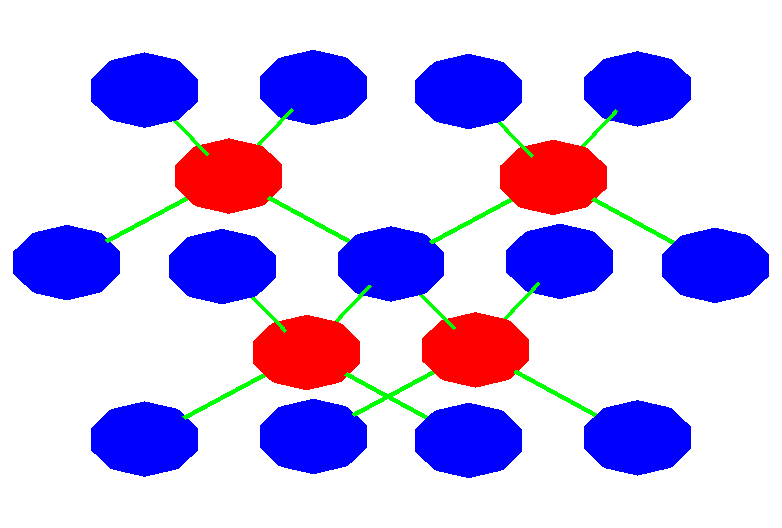
\includegraphics[width=0.35\textwidth]{1_grid3}}%
            \hspace{8pt}%
            %
            \subfloat[][]{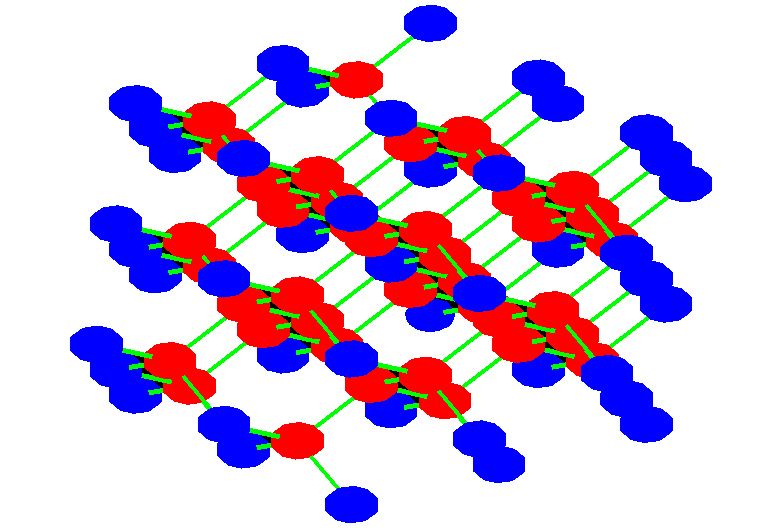
\includegraphics[width=0.35\textwidth]{1_grid5}}%
            \hspace{8pt}%
            %
            \caption[]{Кристаллическая решетка кремния и тремя и пятью слоями соответственно. Синим цветом отмечены внешние атомы.}%
            \label{fig:1}%
        \end{figure}
        %
        \begin{figure}[!htb]%
            \centering
            %
            \subfloat[][]{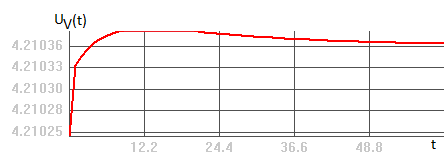
\includegraphics[width=0.45\textwidth]{2_50de}}%
            \hspace{8pt}%
            %
            \subfloat[][]{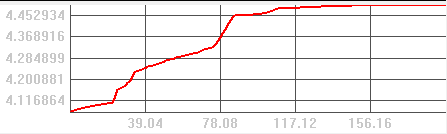
\includegraphics[width=0.45\textwidth]{3_50de}}%
            \hspace{8pt}%
            %
            \subfloat[][]{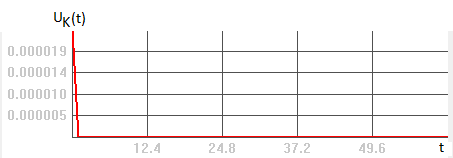
\includegraphics[width=0.45\textwidth]{2_50ek}}%
            \hspace{8pt}%
            %
            \subfloat[][]{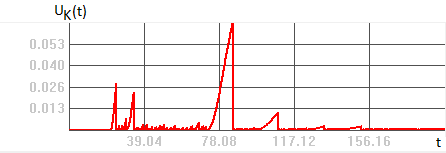
\includegraphics[width=0.45\textwidth]{3_50ek}}%
            \hspace{8pt}%
            %
            \subfloat[][]{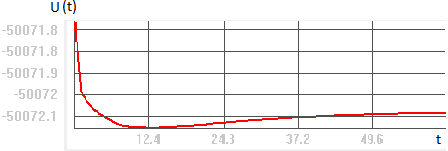
\includegraphics[width=0.45\textwidth]{2_50es}}%
            \hspace{8pt}%
            %
            \subfloat[][]{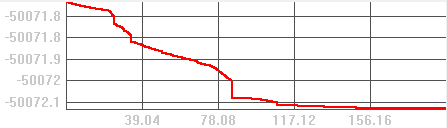
\includegraphics[width=0.45\textwidth]{3_50es}}%
            \hspace{8pt}%
            %
            \subfloat[][]{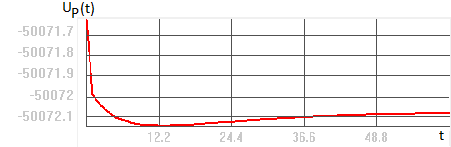
\includegraphics[width=0.45\textwidth]{2_50ep}}%
            \hspace{8pt}%
            %
            \subfloat[][]{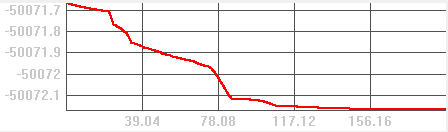
\includegraphics[width=0.45\textwidth]{3_50ep}}%
            \hspace{8pt}%
            %
            \caption[]{Графики установления различных энергий (сверху вниз: энергия образования вакансии, потенциальная, кинетическая, суммарная) при 50 слоях решетки, полученные при жестких (слева) и свободных (справа) граничных условиях. Энергия образования вакансии составила $4.210315$ при жестких и $4.493537$ при свободных граничных условиях.}%
            \label{fig:2}%
        \end{figure}

        Шаг по времени был подобран таким образом, чтобы в процессе моделирования полная энергия системы менялась не сильно (менее $1\%$).

        При разных граничных условиях энергия образования вакансии несколько различается. Это связано с тем, что граничные атомы при разных граничных условиях имеют различное положение в пространстве.

    %
    %
    %
    %%%%%%%%%%%%%%%%%%%%%%%%%%%%%%%%%%%%%%%%%%%%%%%%%%%%%%%%%%%%%%%%%%%%%%%
    %                           SECTION                                   %
    %%%%%%%%%%%%%%%%%%%%%%%%%%%%%%%%%%%%%%%%%%%%%%%%%%%%%%%%%%%%%%%%%%%%%%%
    %
    %
    %

    \section{Выводы}

        В ходе работы была написана демонстрационная программа, позволяющая рассчитывать энергию образования вакансии в кристалле кремния.

        Полученное численное значение энергии образования вакансии оказалось весьма близким к известному ее значению для кремния.


    \clearpage

    \phantomsection
    \addcontentsline{toc}{section}{Список литературы}

    \nocite{*}
    \bibliographystyle{utf8gosttu}
    \bibliography{books}

\end{document}
